\chapter{\IfLanguageName{dutch}{Stand van zaken}{State of the art}}%
\label{ch:stand-van-zaken}

% Tip: Begin elk hoofdstuk met een paragraaf inleiding die beschrijft hoe
% dit hoofdstuk past binnen het geheel van de bachelorproef. Geef in het
% bijzonder aan wat de link is met het vorige en volgende hoofdstuk.

% Pas na deze inleidende paragraaf komt de eerste sectiehoofding.

In dit hoofdstuk wordt de stand van zaken behandeld, ook wel \emph{state of the art} genoemd. Het doel van dit hoofdstuk is om u een overzicht te geven van de meest recente kennis en ontwikkelingen binnen ASR-modellen en machine learning met betrekking tot spraakherkenning. In dit gedeelte wordt voornamelijk ingegaan op modellen en hun werking. Bovendien wordt de relevante terminologie verduidelijkt en uitgelegd. Dit state-of-the-art overzicht biedt de lezer een solide basis om de verdere ontwikkelingen en resultaten in dit onderzoek te begrijpen.
\section{Automatic Speech Recognition}
Automatic speech recognition (ASR) is een technologie die spraakaudio omzet in tekst. Zo bestaan er dan ASR-modellen die de audio analyseren en deze omzetten in een reeks woorden die overeenkomen met wat er werd gezegd. ASR-systemen worden al in verschillende toepassingen gebruikt, namelijk chatbots, automatische translaties in video's en nog veel meer.\autocite{Microsoft2017} Modellen worden getraind met behulp van grote datasets gesproken taal en kunnen daarna geoptimaliseerd worden voor specifieke talen en taken. Gaandeweg zijn er veel kern technologieën ontwikkeld, zoals Gaussiaanse Mixture Models (GMM's), verborgen Markov-modellen (HMM's), mel-frequentie cepstrale coëfficiënten (MFCC's) en hun afgeleiden, ngram-taalmodellen (LM's), discriminerende training. Dit zijn een hele boel technieken die de stand-van-zaken op gebied van ASR enorm verbeterd hebben.\autocite{Mahesha2016}

\subsection{Word Error Rate}
Word Error Rate (WER) is een belangrijke maateenheid die wordt gebruikt om de nauwkeurigheid van ASR-systemen te evalueren. WER is afgeleid van de $\emph{Levenshtein-afstand}$, ook wel bekend als de $\emph{edit distance}$, die de minimale afstand berekent die nodig is om een reeks woorden om te zetten in een andere reeks woorden door middel van toevoegingen, verwijderingen en substituties van woorden. Bij het evalueren van de nauwkeurigheid van een ASR-systeem wordt de WER berekend als de Levenshtein-afstand tussen een gerefereerd woord en zijn automatische transcriptie, genormaliseerd door de lengte van de reeks referentiewoorden. Dit betekent dat de WER de fouten in het automatische transcriptieproces meet als een percentage van het totale aantal woorden in de referentie-uitvoer. Een lage WER duidt op een hoge nauwkeurigheid van het ASR-systeem, terwijl een hoge WER betekent dat er meer fouten zijn opgetreden tijdens het transcriptieproces \autocite{mccowan2004use}. Door gebruik te maken van de WER als evaluatiemaatstaf kan worden bepaald hoe goed een ASR-systeem presteert en kunnen er verbeteringen worden aangebracht om de nauwkeurigheid van het systeem te verbeteren. \\

De definitie van WER gaat als volgt: $N_r$ zijn de totale woorden in de referentie transcriptie, $N_a$ zijn de totale woorden in de transcriptie, S is het aantal vervangen woorden in de automatische transcriptie, D als het aantal woorden uit de referentie verwijderd in de automatische transcriptie, I is het aantal woorden die in de automatische transcriptie zijn ingevoegd en niet in de referentie voorkomen en H als het aantal correct herkende woorden. Zo kunnen we dan de woord error rate definiëren als: \par 
\[WER = \frac{S + D + I}{N_r}.\]
Dit wordt het meest gebruikt als error verhouding, je kunt aan de hand van WER ook de word recognition rate (WRR) bereken: \par
\[WRR = 1 - WER = \frac{H-I}{N_r} .\]
Soms wordt er ook gebruik gemaakt van de word correct rate (WCR), deze maateenheid maakt geen gebruik van inserties en errors en wordt gedefinieerd als volgt: \par
\[WCR = \frac{H}{N_r} .\] \autocite{mccowan2004use}  
Verduidelijking aan de hand van een voorbeeld: 
\begin{quote}
    Referentietekst: "Het is een zonnige dag vandaag."\\
    Herkende tekst: "Het is een regenachtige dag vandaag."
\end{quote}
Nu wordt er berekend hoe veel invoegingen (I), verwijderingen (D) en substituties (S) er nodig zijn om da herkende tekst overeen te laten komen met de referentietekst:
\begin{quote}
Invoegingen (I): Geen\\
Verwijderingen (D): Geen\\
Substituties (S): `regenachtig' in plaats van 'zonnige'
\end{quote}
Het totale aantal woorden ($N_r$) is 6, dus als we dan de formule volgen ziet dit er als volgt uit:
\[WER = \frac{S + D + I}{N_r} = \frac{1+0+0}{6}.\]
\[WER ≈ 0.1667\]
In dit voorbeeld wordt er een word error rate van ongeveer 0.1667 berekend. Dit wil zeggen dan 16.67\% van de woorden in de herkende tekst afwijkt van de referentietekst.
\subsection{Self-supervised Learning}
In het domein machine learning is self-supervised learning naar voren gekomen als een paradigma om algemene gegevens te leren. Normaal gesproken wordt bij supervised training gebruik gemaakt van data dat gelabeld is. Het probleem is dat ook al is er veel beschikbare data, je kunt pas gebruik maken van supervised learning als deze data gelabeld is. Bij self-supervised learning worden de labels zelf gegenereerd waardoor er geen door mensen geannoteerde labels nodig zijn \autocite{Jaiswal2021}. ASR-systemen zoals Whisper en Wav2Vec gebruik maken van  self-supervised learning. Waardoor het mogelijk wordt gebruik te maken van de grote hoeveelheid ongelabelde gegevens die beschikbaar zijn.

\subsection{Whisper}
Whisper is een ASR-systeem dat in 2022 werd ontwikkeld door OpenAI.
Het is getraind op 680.000 uur aan meertalige gegevens die via het internet zijn verzameld. Door gebruik te maken van grote en diverse data leidt tot verbeterde robuustheid voor accenten, achtergrondgeluiden en technisch taalgebruik\autocite{OpenAI2022}. Om deze reden zou Whisper een geschikte ASR-systeem kunnen zijn voor dit onderzoek.

\subsubsection{Whisper structuur}
De architectuur van Whisper heeft een end-to-end benadering, geïmplementeerd als encoder-decoder transformer. De ingevoerde audio wordt opgesplitst in stukken van 30 seconden. Deze stukken worden dan omgezet in een log-Mel-spectogram wat vervolgens wordt doorgegeven aan een encoder, op figuur \ref{fig:spec} ziet u een voorbeeld van een log-Mel spectogram. Veder gaat dan een getrainde decoder de corresponderende tekstonderschrift voorspellen \autocite{OpenAI2022}. Op figuur \ref{fig:whisp} is een duidelijk overzicht weergegeven van de structuur van Wisper.
\begin{center}
    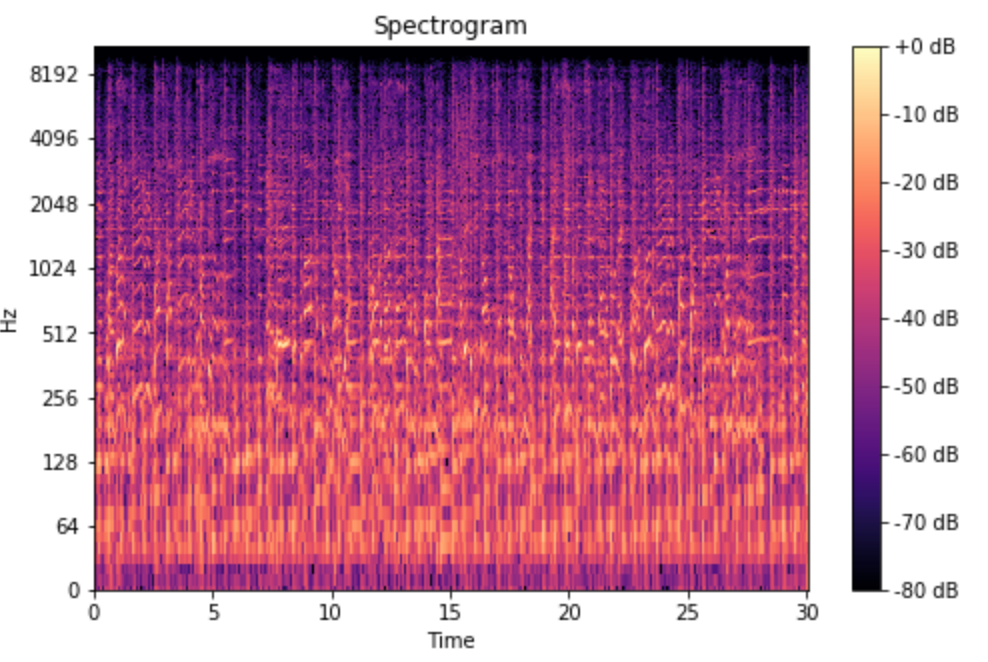
\includegraphics[scale=0.25]{logMelSpec}
    \captionof{figure}{Voorbeeld van een log-mel spectogram, dit geeft een signaal weer op een frequentiespectrum. \autocite{mel-spectrogram-medium}}
    \label{fig:spec}
\end{center}
\begin{center}
    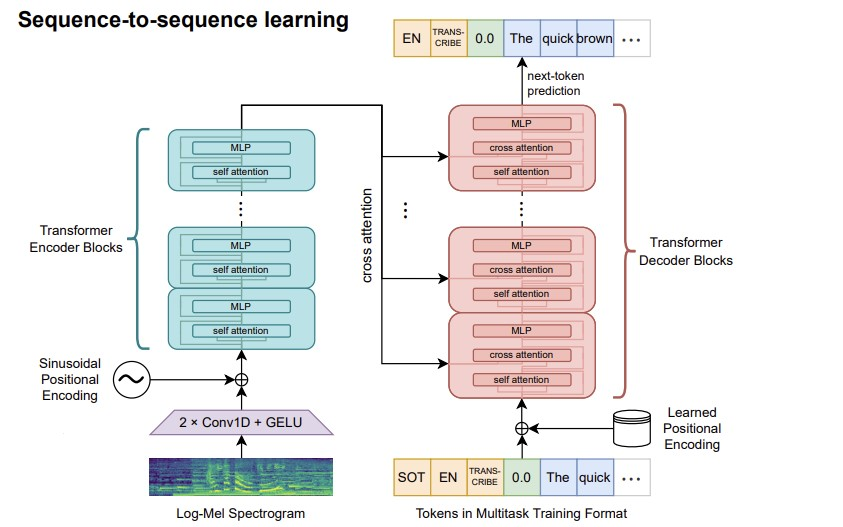
\includegraphics[scale=0.75]{whisper}
    \captionof{figure}{Overzicht van de structuur van het Whisper asr-systeem. \autocite{Tjandra2020}}
    \label{fig:whisp}
\end{center}

\subsubsection{Nederlandse taal}
Whisper is in staat om meerdere talen te begrijpen, waaronder het Nederlands. Whisper heeft verschillende modellen van verschillende groottes, en de prestaties kunnen sterk variëren tussen deze modellen. Het Whisper large-v2-model presteert het beste voor de Nederlandse taal. Bij de Common Voice 9-dataset behaalt het een WER van 5,8\% en bij de Librispeech-dataset een WER van 9,3\% \autocite{Tjandra2020}.

\subsection{Wav2Vec 2.0}
Wav2Vec 2.0 is een framework voor spraakherkenning dat is gemaakt door Facebook AI Research (FAIR). Het is heel populair geworden in de ASR-wereld omdat het heel opmerkelijke prestaties levert. De reden waarom Wav2Vec 2.0 zo goed presteert is omdat het framework zich richt op de raw waveform van de spraak \autocite{baevski2020wav2vec}. Dus in plaats van de audio om te zetten werken ze rechtstreeks met de audio van spraaksignalen. 

\subsubsection{Wav2Vec 2.0 structuur}
Het model is samengesteld uit een Convolutional Neutral Network (CNN), ook wel de feature encoder genoemd, die de raw onbewerkte audio (X) neemt en het levert van latente spraakrepresentaties (z1, z2, ..., zT) voor T tijdsstappen. Vervolgens worden deze dan gevoerd aan een transformer. Deze transformer maakt dan representaties (c1, c2, ..., cT), bij deze stap wordt er ook informatie uit de gehele sequentie vastgelegd. De output van de feature encoder wordt dan gediscretiseerd met een quantization module om het representeren van een doel in het self-supervised learning \autocite{baevski2020wav2vec}. In figuur \ref{fig:wav2vec} zie je een visueel beeld van de structuur van het Wav2Vec 2.0 model.

\begin{center}
    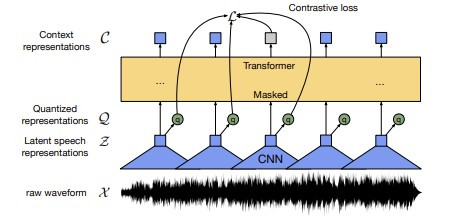
\includegraphics{Wav2Vec}
    \captionof{figure}{Visuele illustratie van de Wav2Vec 2.0 structuur \autocite{baevski2020wav2vec}.}
    \label{fig:wav2vec}
\end{center}

\subsubsection{Performantie}
Natuurlijk wanneer je een spraakherkenningsmodel wilt gebruiken moet je ook kijken naar de prestatie die het kan leveren. Wanneer Wav2Vec 2.0 getest wordt op de LibriSpeech dataset dan krijgen we goede resultaten weer. Bij de 10 minuten gelabelde data presteert het een Word Error Rate (WER) van 4.8\% en bij ongelabelde is het 8.2\%. Hiervoor moest het model natuurlijk eens getraind worden, dit werd gedaan door het 53 duizend uur ongelabelde data van de LibriVox dataset \autocite{baevski2020wav2vec}. 

\subsubsection{Nederlands model}
Wav2vec2-large-xlsr-53-dutch is gemaakt door Jonatas Grosman, een professor aan de katholieke universiteit van Rio de Janeiro. Zijn model is getest geweest met de Common Voice dataset en Collection of Single Speeker (CSS) dataset. Op deze datasets behaalde het een WER van 15.72\% \autocite{grosman2021xlsr53-large-dutch}.\\
Het maakt gebruik van XLSR, een taalmodel is dat gemaakt door Huggingface en Facebook \autocite{2022}. Het doel hiervan is om modellen te trainen die meerdere talen begrijpen en te kunnen verwerken. In tegenstelling tot traditionele taalmodellen, die meestal getraind zijn op één taal, kunnen XLSR-modellen meerdere talen bevatten en kunnen worden afgestemd op een specifieke talen om zo de prestatie van die talen te verbeteren \autocite{2021}.

\section{Stotter Correctie}
Wanneer iemand een ASR model gebruikt en onvloeiend spreekt dan heeft het model moeite met het correct te transcriberen. Gelukkig kan er gebruikt worden van stotter correctie. In 2020 hebben studenten van PES University in India een automatische correctie methode van onvloeibare spraak uitgewerkt. Er wordt gebruik gemaakt van Mel Frequency Cepstral Coefficients (MFCC) en Linear Predictive Coefficients \autocite{KN2020}.

\subsection{Mel Frequency Cepstral Coefficients}
Mel Frequency Cepstral Coefficients is een concept voor het extraheren van kenmerken van een akoestisch signaal. Het is gebaseerd op de frequenties van meer dan 1KHz, dus wat het menselijk gehoor niet meer kan waarnemen. De berekeningen die door MFCC worden uitgevoerd zijn zeer afhankelijk van het proces waarbij de signalen veranderen van analoog naar digitaal. MFCC voert berekeningen uit variërend van de lengte van de golfhoogte, ruis en andere dingen zodat de woorden die werden uitgesproken door de gebruiker worden verkregen \autocite{haq2020speech}.

\subsection{Linear Predictive Coefficients}
Linear Predictive Coding (LPC) is een techniek die wordt gebruikt in audioprocessing en spraakanalyse om de spectrale eigenschappen van een signaal te modelleren. De techniek is gebaseerd op het idee dat het spectrum van een signaal kan worden voorspeld door gebruik te maken van een lineair voorspellingsmodel. Bij LPC wordt het signaal opgedeeld in korte stukjes en wordt er voor elk stukje een set lineaire predictieve coëfficiënten berekend. Deze coëfficiënten worden gebruikt om een lineair voorspellingsmodel te bouwen, dat vervolgens kan worden gebruikt om het spectrum van het signaal te modelleren en te analyseren. De LPC-techniek wordt veel gebruikt in spraaktechnologie, bijvoorbeeld om spraak te comprimeren of om spraak te herkennen in een spraakherkenningssysteem. Het is ook een belangrijk onderdeel van codecs zoals MP3 en AAC, die worden gebruikt voor het comprimeren van audiobestanden. \autocite{bradbury2000linear}. 
 
\subsection{Design}
Het design bestaat uit een sequentie van drie algoritmen. Het eerste algoritme is voor het verwijderen van herhaling, dus worden alle gerepeteerde woorden geëlimineerd en behoudt alle niet-herhaalde woorden. Dit wordt behaald door gebruik MFCC- en LPC-functies van 2 opeenvolgende woorden te extraheren. Als er dan een hoge correlatie is tussen de geëxtraheerde kenmerken van de 2 woorden duidt op een grote gelijkenis tussen woorden, waarna het herhaalde woord wordt geëlimineerd.\\

Er is ook een algoritme voor het verwijderen van lange pauzes in de audio. Dit wordt gedaan door het berekenen van de tijd tussen het einde van een woord en het begin van het opeenvolgende woord. Wanneer dit dan meer dan 0.5s is impliceert dit op een lange pauze.\\

Uiteindelijk is er dan ook een verlenging verwijdering aan de hand van een algoritme. Hierbij wordt het audio fragment opgedeeld in in frames van 50ms. Dan wordt er rekening gehouden met de MFCC- en LPC-kenmerken die overeenkomen met opeenvolgende frames en wordt er een correlatiefactor gevonden. Deze factor wordt achterhaald tussen kenmerken van opeenvolgende frames. Bij een langdurig optreden van hoge correlatie tussen frames impliceert dit dat er een verlenging is (bijvoorbeeld: sttttttttop) \autocite{KN2020}.

\subsection{Performantie}
De algortimen zijn effectief in staat om lange pauzes, verlengingen en herhalingen te herkennen en te corrigeren. Bij de 80 instanties van lange pauzes heeft het algoritme 78 keer de pauzes herkend, dat is een accuraatheid van 97.5\%. Bij het testen op herkenning van verlengingen en herhalingen bevatte de audiobestanden in totaal 60 herhalings- en 70 verlengingsgebeurtenissen. Hierbij werden 2 verschillende functies gebruikt: MFFC en LPC. In figuur \ref{fig:tabel} kunt u zien dat MFCC accurater is dan LPC. MFCC behaalde een gemiddelde nauwkeurigheid van 92.8\% en LPC een 89.9\% \autocite{KN2020}

\begin{center}
    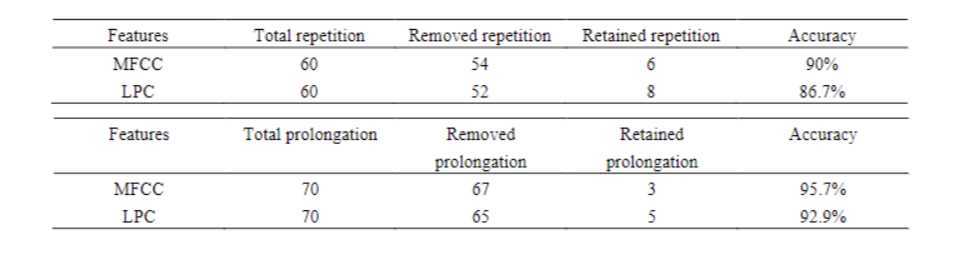
\includegraphics[width = 5in]{tabellen_MFCC_LPC}
    \captionof{figure}{Tabel dat overzicht geef over de accuraatheid van de functies (MFCC, LPC). \autocite{KN2020} }
    \label{fig:tabel}
\end{center}
 